\usetikzlibrary{backgrounds,calc}

\begin{document}
	\chapter{Probability}
	\section{Introduction}
	Let an event be denoted by $A$. The probability that event $A$ occurs is denoted by P$(A)$ and is given by \[\Pr(A) = \frac{\text{no. of ways in which } A \text{ can occur}}{\text{total no. of outcomes}}\]
	
	Also note that the probability of event $A$ not happening is defined by $1-\Pr(A)$ and is denoted by $\Pr(A^c)$.
	
	\begin{example}
		A letter is chosen at random from the world `CALCULUS'. Find the probability that it is:
		
		\quad \textbf{a) } a `C'.
		
		\quad \textbf{b) } a vowel.
	\end{example}

\begin{example}
	A card is chosen at random from a pack of 52 playing cards. Find the probability that the card is: 
	
	\quad \textbf{a) } an ace.
	
	\quad \textbf{b) } black.
	
	\quad \textbf{c) } a heart.
	
	\quad \textbf{d) } a royal card.
\end{example}
	\section{Using Permutations and Combinations}
	
	In the following problem, the number of successful outcomes and the total number of outcomes are calculated using the counting techniques in the previous chapter.
	
	\begin{example}
		A team of 6 children is chosen at random from a class of 10 girls and 9 boys. Find the probability thattge selected team contains:
		
		\quad \textbf{a) } girls only.
		
		\quad \textbf{b) } boys only.
			
		\quad \textbf{c) } more girls than boys.
		
		\quad \textbf{d) } the oldest 5 children in the class.
		
	\end{example}
	\section{Bernoulli Trials}
	A Binomial Experiment is an experiment which satisfies the following 4 conditions:
	\begin{itemize}
		\item {A fixed number of trials.}
		\item {Each trial is independent of the others.}
		\item {There are only \textbf{two} outcomes.}
		\item {The probability of each outcome remains constant from trial to trial.}
	\end{itemize}
	\section{Probability Space Diagrams and Tree Diagrams.}
	Tree diagrams and possibility spaces are simple graphical tools which help us calculate probabilities. Possibility space diagrams are particularly useful when the problem involves independent events.
	\section{Venn Diagrams}
	Venn diagrams ilustrate sets of objects or items and set operations. Consider for instance the sets $M_2$, $M_3$ and $M_5$ which stand for multiples of 2, 3 and 5 respectively. The \textbf{universal} set $U$ is the set of all integers between 1 and 30. For convenience, let us consider the set $P$ to be the set of all primes between 1 and 30.
	
	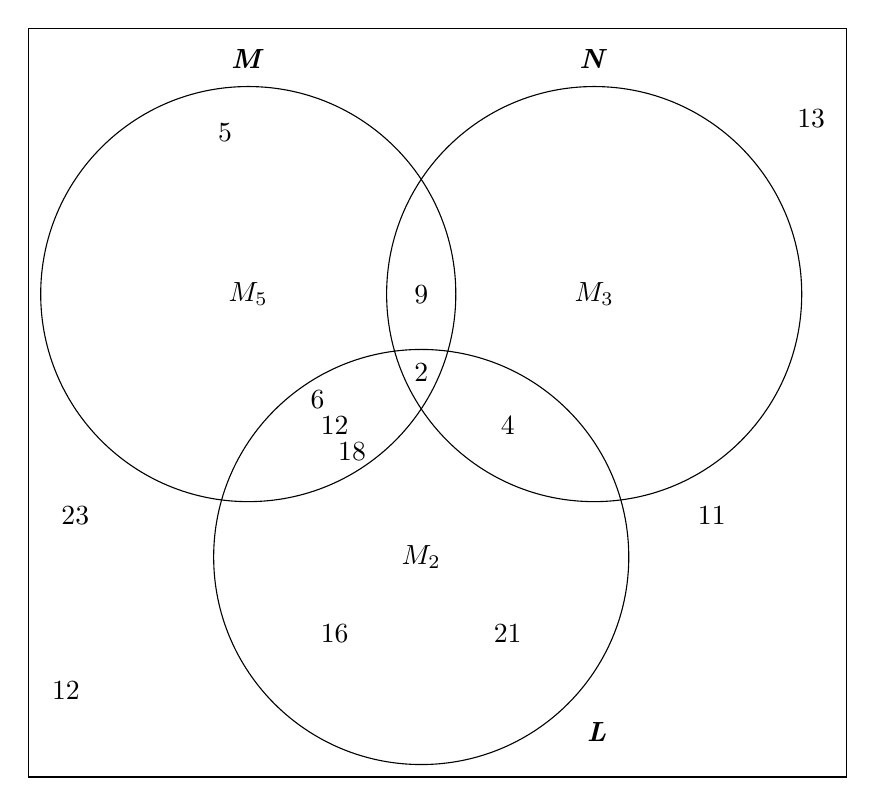
\begin{tikzpicture}[venncircle/.style={draw, circle, minimum size=15em, align=center}, node distance=12.5em, framed] 
		\node[venncircle] (circle1) {$M_5$};    
		\node[venncircle, right of=circle1] (circle2) {$M_3$};
		\node (MN) at ($(circle1)!0.5!(circle2)$){9};
		\node[venncircle, below of=MN, yshift=3em] (circle3) {$M_2$}; %yshift value by pythagoras
		\node (ML)  at ($(circle1)!0.4!(circle3)$){6};
		\node (ML)  at ($(circle1)!0.5!(circle3)$){12};
		\node (MLa)  at ($(circle1)!0.6!(circle3)$){18};    
		\node (NL)  at ($(circle2)!0.5!(circle3)$){4};   
		\node (MNL)  at ($(MN)!0.3!(circle3)$){2};
		\node (Lleft) [below of=ML, yshift=5em] {16};
		\node (Lright) [below of=NL, yshift=5em] {21};
		\node (outbotrightnum) [right of=circle3, yshift=1.5em, xshift=-2em] {11};
		\node (outtoprightnum) [above right of=circle2, yshift=-2.5em, xshift=-1em] {13};
		\node (outbotleftnum) [below left of=circle3, yshift=4em, xshift=-4em]{12};
		\node (outtopleftnum) [left of=circle3, yshift=1.5em]{23};
		\node (U)[above left of=circle1, xshift=8em, yshift=-3em]{5};
		\node (M)[above of=circle1, yshift=-4em]{\textbf{\textit{M}}};
		\node (N)[above of=circle2, yshift=-4em]{\textbf{\textit{N}}};
		\node (L)[below right of=circle3, yshift=2.5em, xshift=-2.5em]{\textbf{\textit{L}}};
	\end{tikzpicture}  
\begin{itemize}
	\item{The intersection between sets $M_2$ and $M_3$ is denoted by $M_2 \cap M_3$ and hence $M_2 \cap M_3 = \set{6,12,18,25,30}$ and $M_2 \cap M_3 \cap M_5 = \set{30}$.}
	
	\item{The union between the sets $M_3$ and $M_5$ is denoted by $M_3 \cup M_5$ and hence $M_3 \cup M_5 = \set{3,5,6,7,10,12,15,18,20,21,24,25,27,30}$.}
	
	\item{We already know that the set that is formed by the members of the universal set which are not in the set $M_2$ is called the complement of the set $M_2$ denoted by $M_2^c$. Hence, $M_2^c = \set{1,3,5,7,9,11,13,15,17,19,21,23,25,27,29}$.}
\end{itemize}






We already know that the set that is formed by the members of the universal set which are not in the set $M_2$ is called the complement of the set $M_2$ denoted by $M_2^C$

\end{document}